
\documentclass[
	11pt,
]{beamer}

\graphicspath{{Images/}{./}} 

\usepackage{booktabs} 

%----------------------------------------------------------------------------------------
%	SELECT LAYOUT THEME
%----------------------------------------------------------------------------------------

\usetheme{CambridgeUS}

%----------------------------------------------------------------------------------------
%	SELECT COLOR THEME
%----------------------------------------------------------------------------------------

\usecolortheme{seahorse}

%----------------------------------------------------------------------------------------
%	SELECT FONT THEME & FONTS
%----------------------------------------------------------------------------------------

\usefonttheme{default} % Typeset using the default sans serif font

%------------------------------------------------

\usepackage{palatino} % Use the Palatino font for serif text

\usepackage[default]{opensans} % Use the Open Sans font for sans serif text

%----------------------------------------------------------------------------------------
%	SELECT INNER THEME
%----------------------------------------------------------------------------------------

\useinnertheme{circles}

%----------------------------------------------------------------------------------------
%	PRESENTATION INFORMATION
%----------------------------------------------------------------------------------------

\title[Lorenz System and Parareal]{ \text{Exploring Chaos Theory} \\ \textbf{The Lorenz System and Parareal Algorithm}}


\author[O. BOUHENNICHE \and N. ZAOUACHE]{Oussama BOUHENNICHE \and Narimane ZAOUACHE}

\institute[]{University of Strasbourg}


\date[\today]{ CSMI \\ \today}

%----------------------------------------------------------------------------------------

\begin{document}

%----------------------------------------------------------------------------------------
%	TITLE SLIDE
%----------------------------------------------------------------------------------------

\begin{frame}
	\titlepage
\end{frame}

%----------------------------------------------------------------------------------------
%	PRESENTATION BODY SLIDES
%----------------------------------------------------------------------------------------

\section{Chaos Theory and Lorenz System} 

%------------------------------------------------
\begin{frame}
    \frametitle{Chaos Theory and Lorenz System}
	\begin{columns}[c]
		\begin{column}{0.65\textwidth} 
			\begin{itemize}
				\item Definition of chaos theory.
				\item Introduction of the butterfly effect concept.
				\item Aiming to explore how tiny causes lead to huge effects in chaotic systems.
				\item Aiming to explore Lorenz system and Parareal algorithm.
			\end{itemize}
		\end{column}
		\begin{column}{0.35\textwidth}
			\begin{figure}
				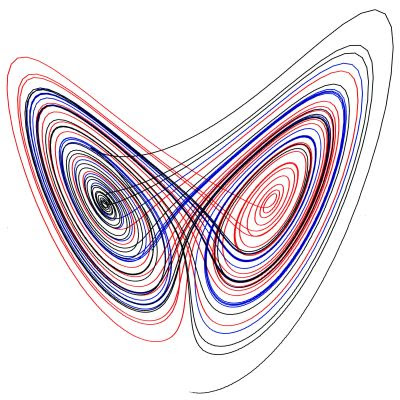
\includegraphics[width=1\linewidth]{butterfly.jpg}
			\end{figure}
		\end{column}
	\end{columns}

\end{frame}

%------------------------------------------------

\section{Roadmap}
\begin{frame}
    \frametitle{Roadmap}
	\begin{columns}[c]
		\begin{column}{\textwidth}
			\begin{itemize}
				\item Brief overview of project objectives.
				\item Steps: Implementing Lorenz Model, studying ODE solvers, exploring Parareal algorithm
				\item Emphasis on iterative and comparative nature of the project
			\end{itemize}
		\end{column}
	\end{columns}
\end{frame}

%------------------------------------------------

\section{Conclusion}

\begin{frame}
	\frametitle{Conclusion}
	\begin{center}
		{\Huge The End}

		\bigskip\bigskip

		{\LARGE Questions? Comments?}
	\end{center}
\end{frame}

%----------------------------------------------------------------------------------------

\end{document}